%\chapter{Appendix A} % Main appendix title
\appendix
\chapter{Projected Density of States of C--S--H} % Main appendix title
\label{AppendixA} % For referencing this appendix elsewhere, use \ref{AppendixA}


\begin{figure}[h]
    \centering
    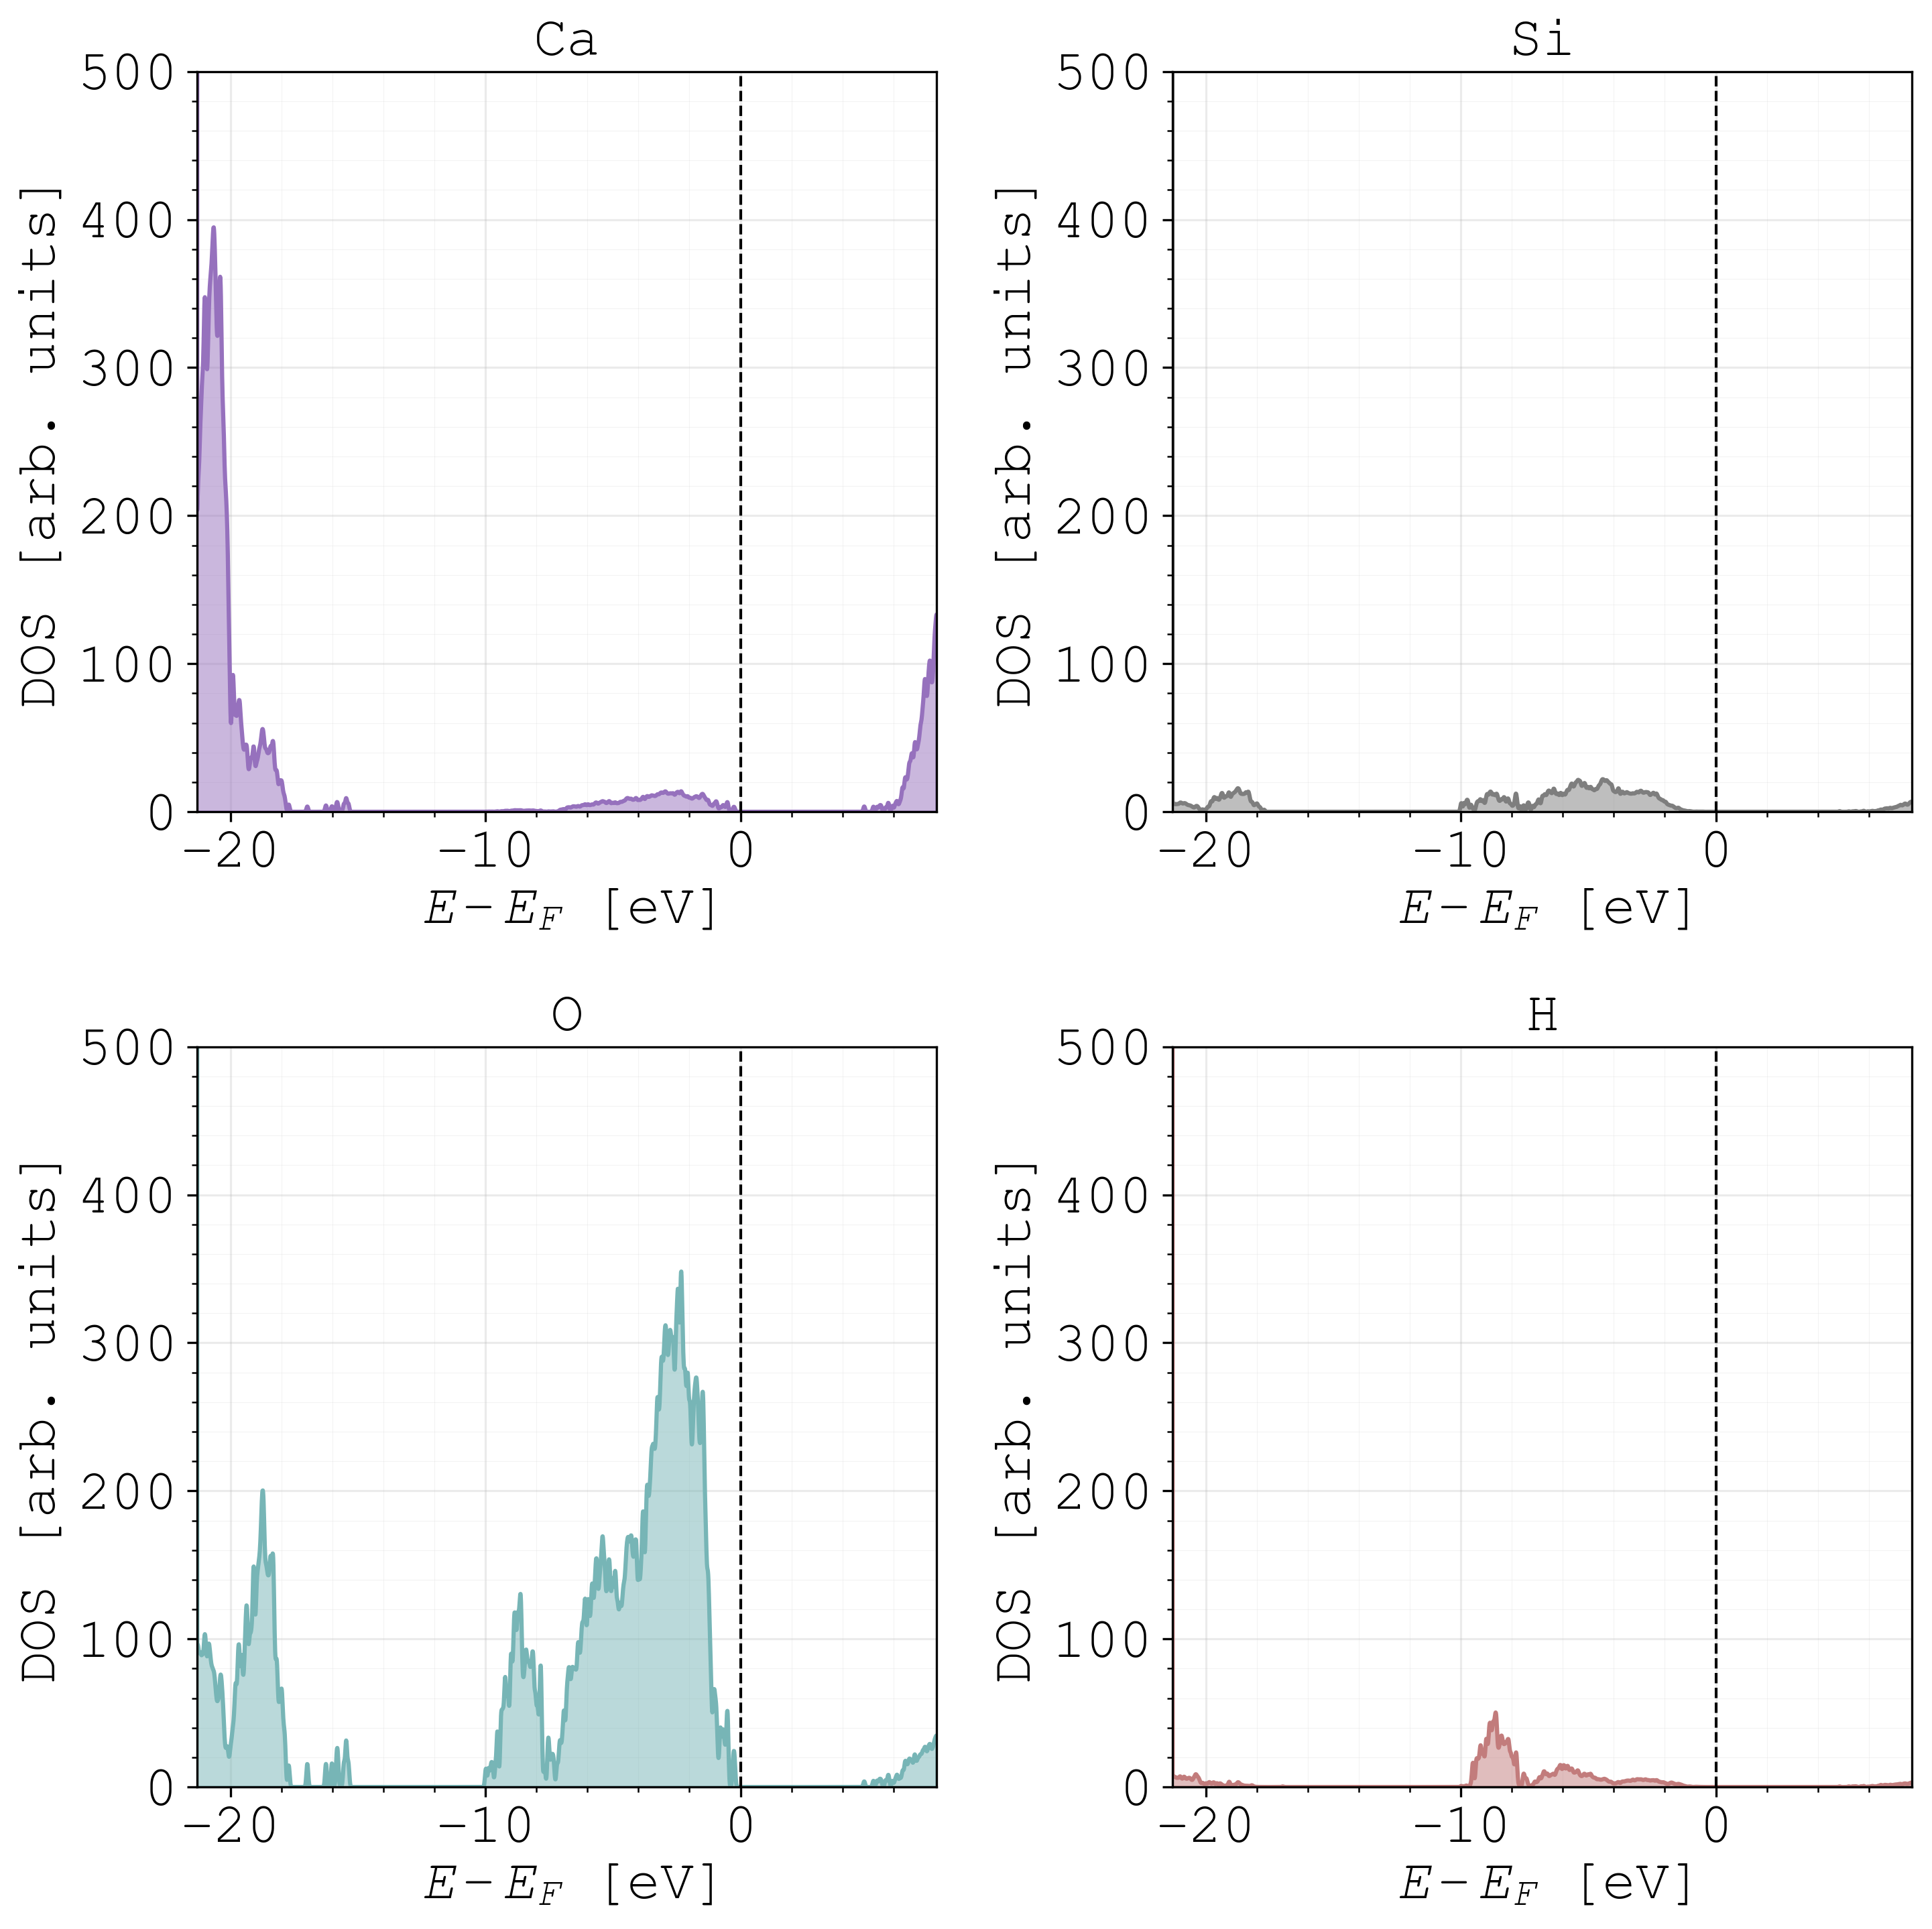
\includegraphics[width=0.8\textwidth]{dos-per-element.png}
    \caption{
        Detailed electronic density of states (DOS) of C--S--H computed using the HSEsol hybrid functional. Element-resolved contributions from Ca, Si, O, and H are shown. The energy axis (x-axis) is referenced to the Fermi level, indicated by the dashed vertical line at 0 eV, while the y-axis represents the density of states (in states/eV).}
    \label{fig:pdos-all}
\end{figure}

\begin{figure}[h]
    \centering
    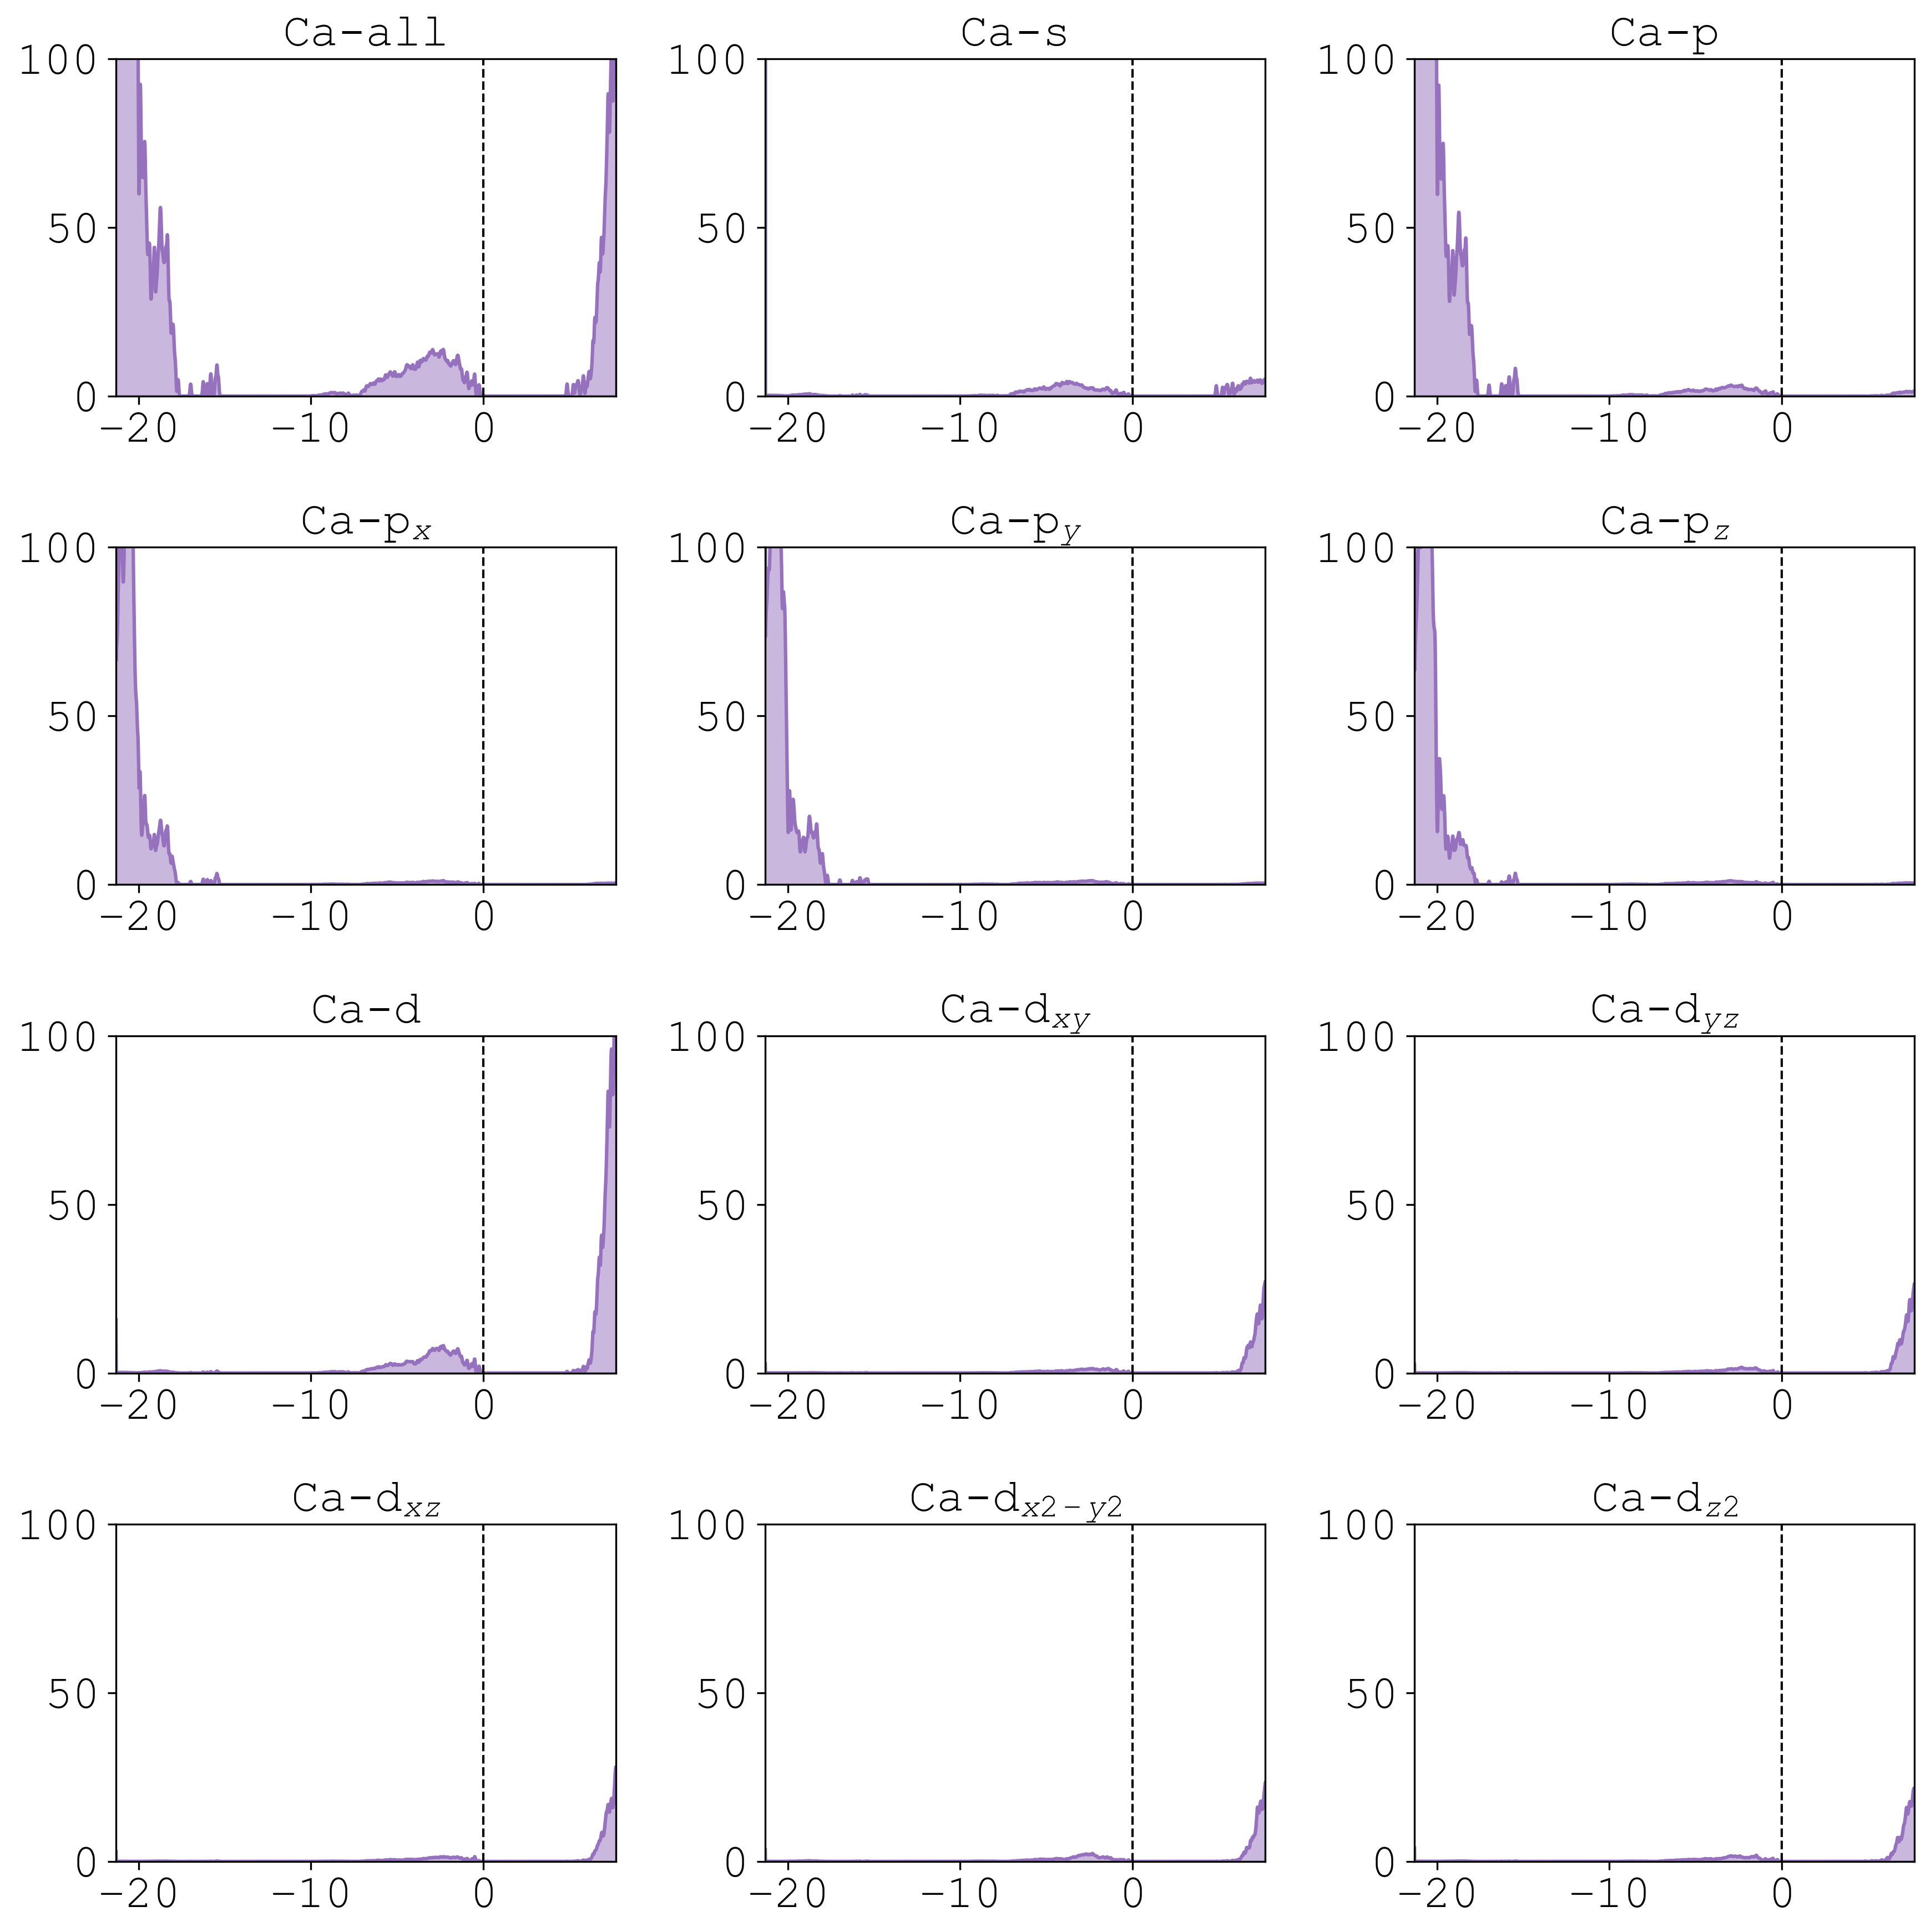
\includegraphics[width=1.0\textwidth]{dos-ca-orbitals.png}
    \caption{Orbital-resolved density of states (DOS) for Ca atoms in C--S--H computed employing the HSEsol hybrid functional. The plots show the total Ca contribution and its decomposition into \textit{s}, \textit{p} (\textit{p}$_x$, \textit{p}$_y$, \textit{p}$_z$), and \textit{d} (\textit{d}$_{xy}$, \textit{d}$_{yz}$, \textit{d}$_{xz}$, \textit{d}$_{x^2-y^2}$, \textit{d}$_{z^2}$) orbitals. The x-axis reports the energy (in eV) relative to the Fermi level (dashed vertical line at 0 eV), while the y-axis shows the density of states (in states/eV).}
    \label{fig:pdos-ca}
\end{figure}

\begin{figure}[h]
    \centering
    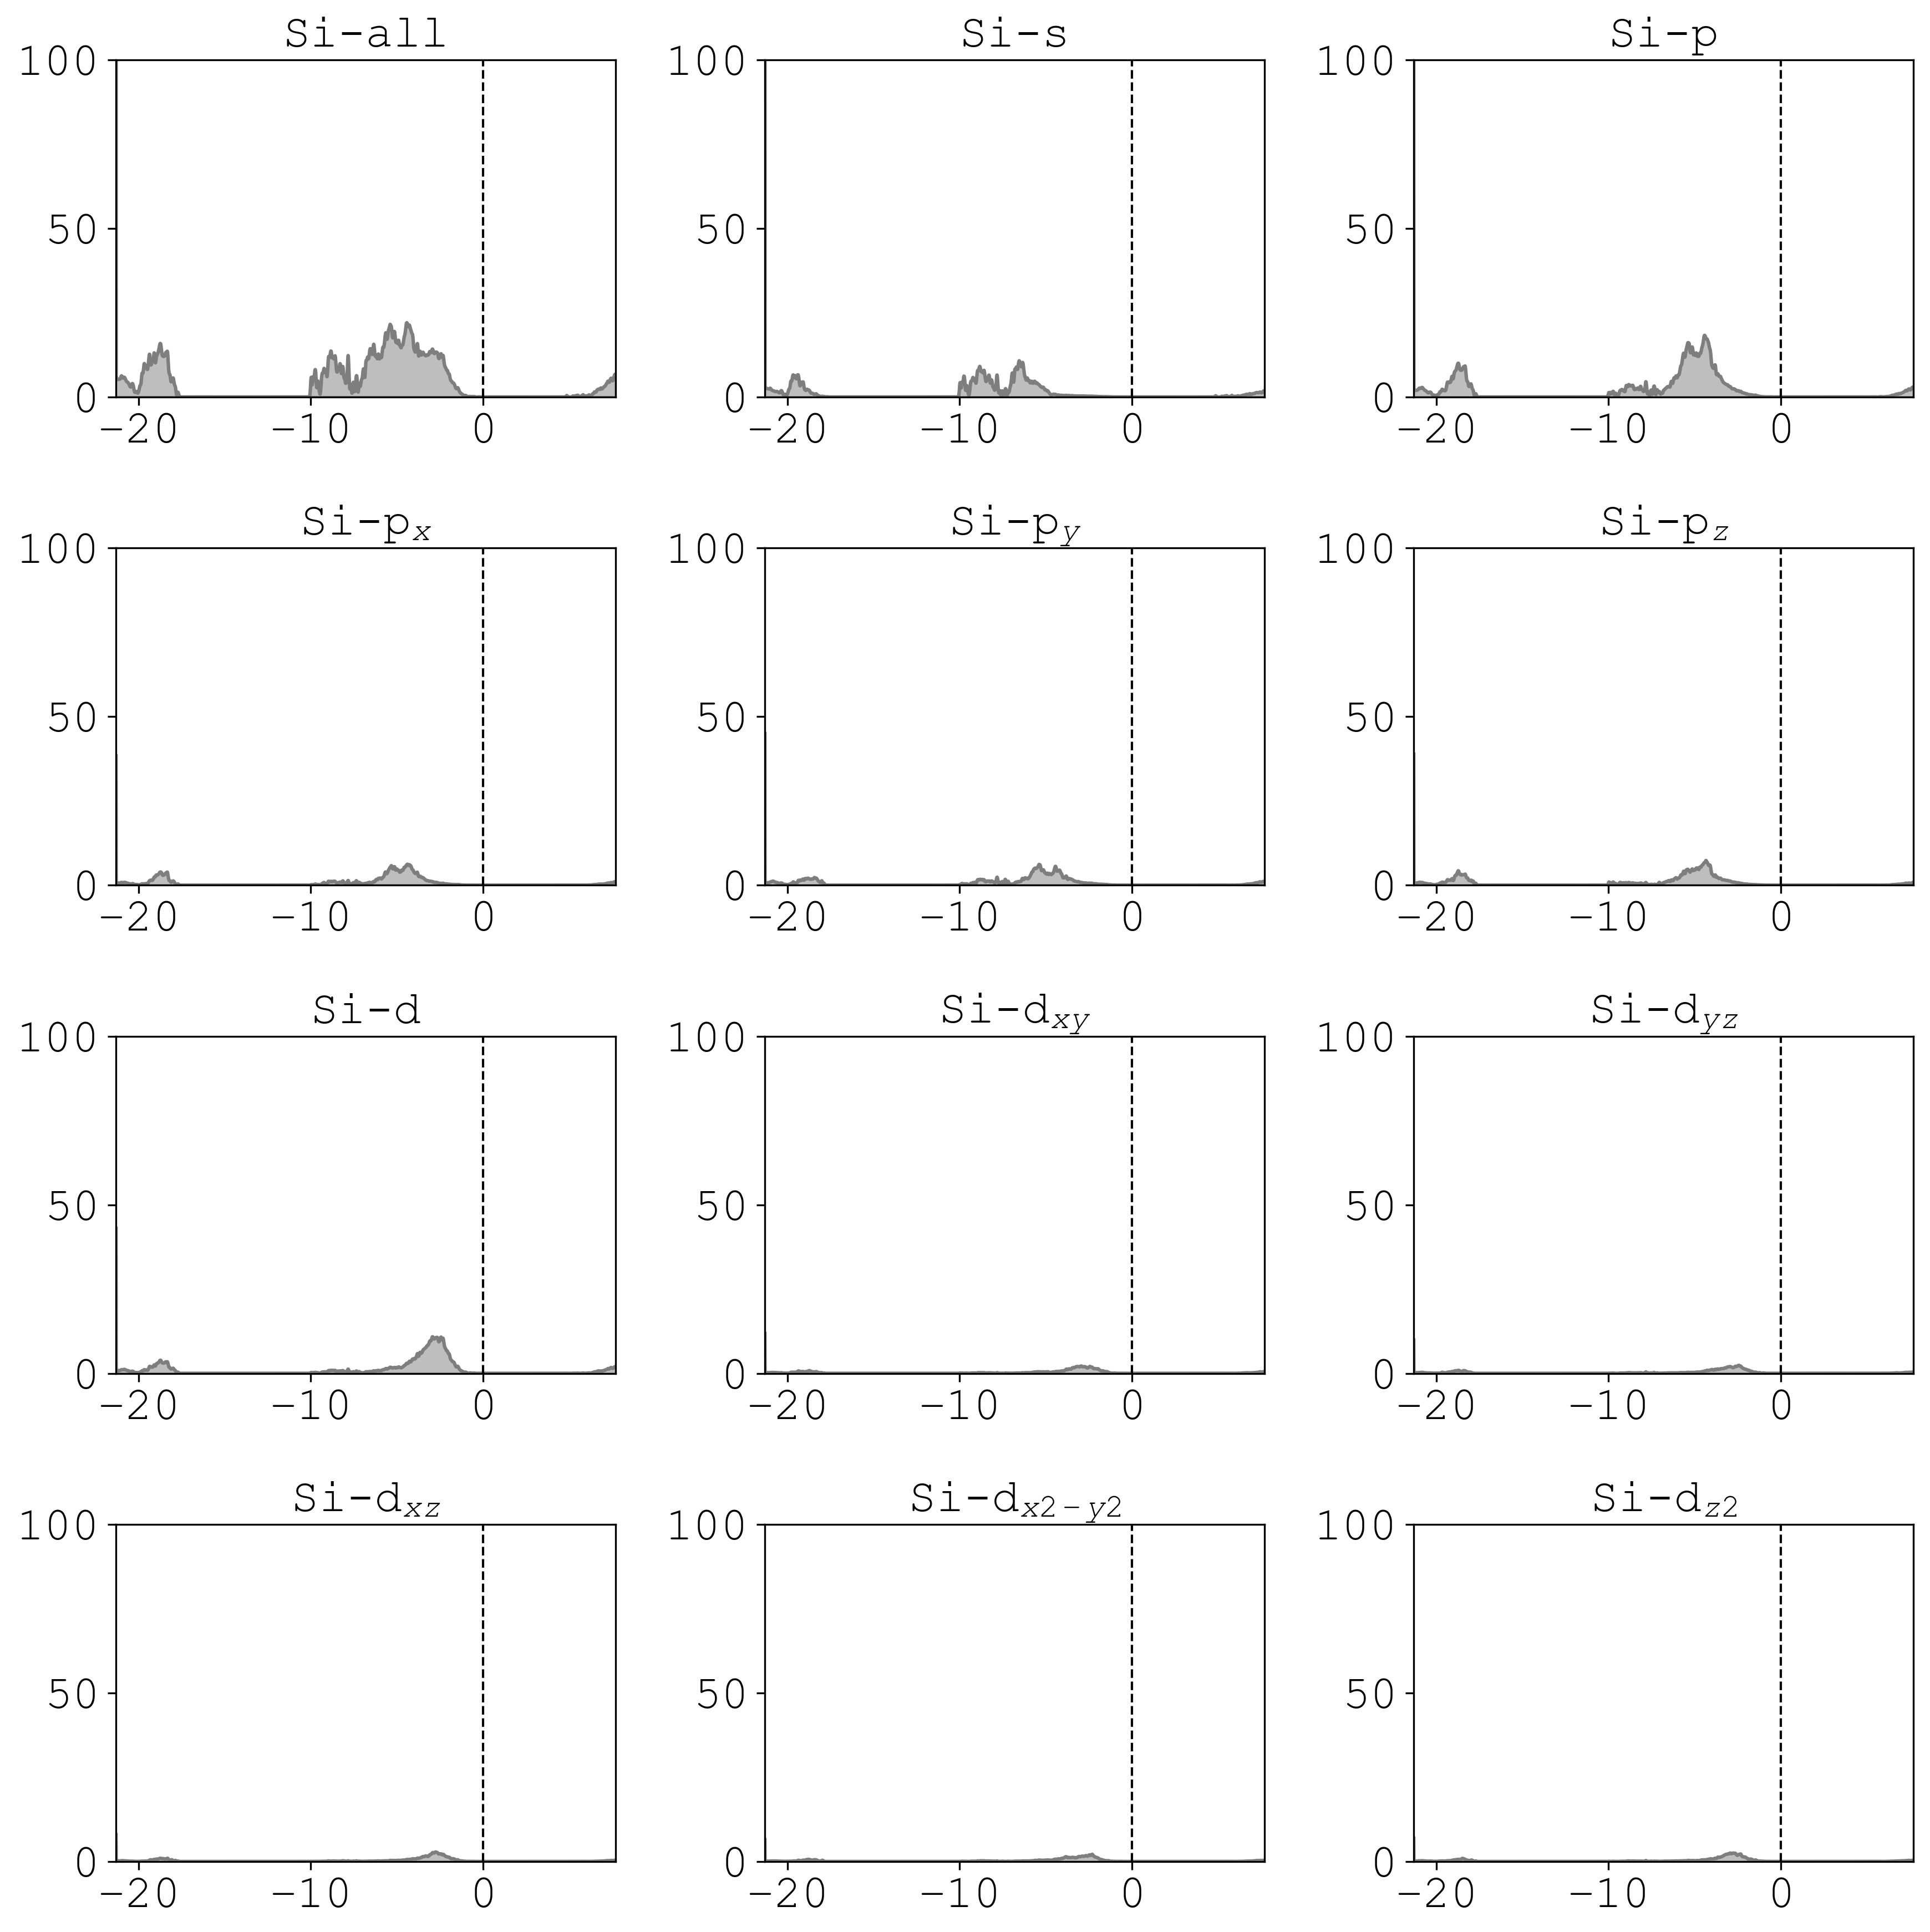
\includegraphics[width=1.0\textwidth]{dos-si-orbitals.png}
    \caption{Orbital-resolved density of states (DOS) for Si atoms in C--S--H computed employing the HSEsol hybrid functional. The plots show the total Si contribution and its decomposition into \textit{s}, \textit{p} (\textit{p}$_x$, \textit{p}$_y$, \textit{p}$_z$), and \textit{d} (\textit{d}$_{xy}$, \textit{d}$_{yz}$, \textit{d}$_{xz}$, \textit{d}$_{x^2-y^2}$, \textit{d}$_{z^2}$) orbitals. The x-axis reports the energy (in eV) relative to the Fermi level (dashed vertical line at 0 eV), while the y-axis shows the density of states (in states/eV).}
    \label{fig:pdos-si}
\end{figure}

\begin{figure}[h]
    \centering
    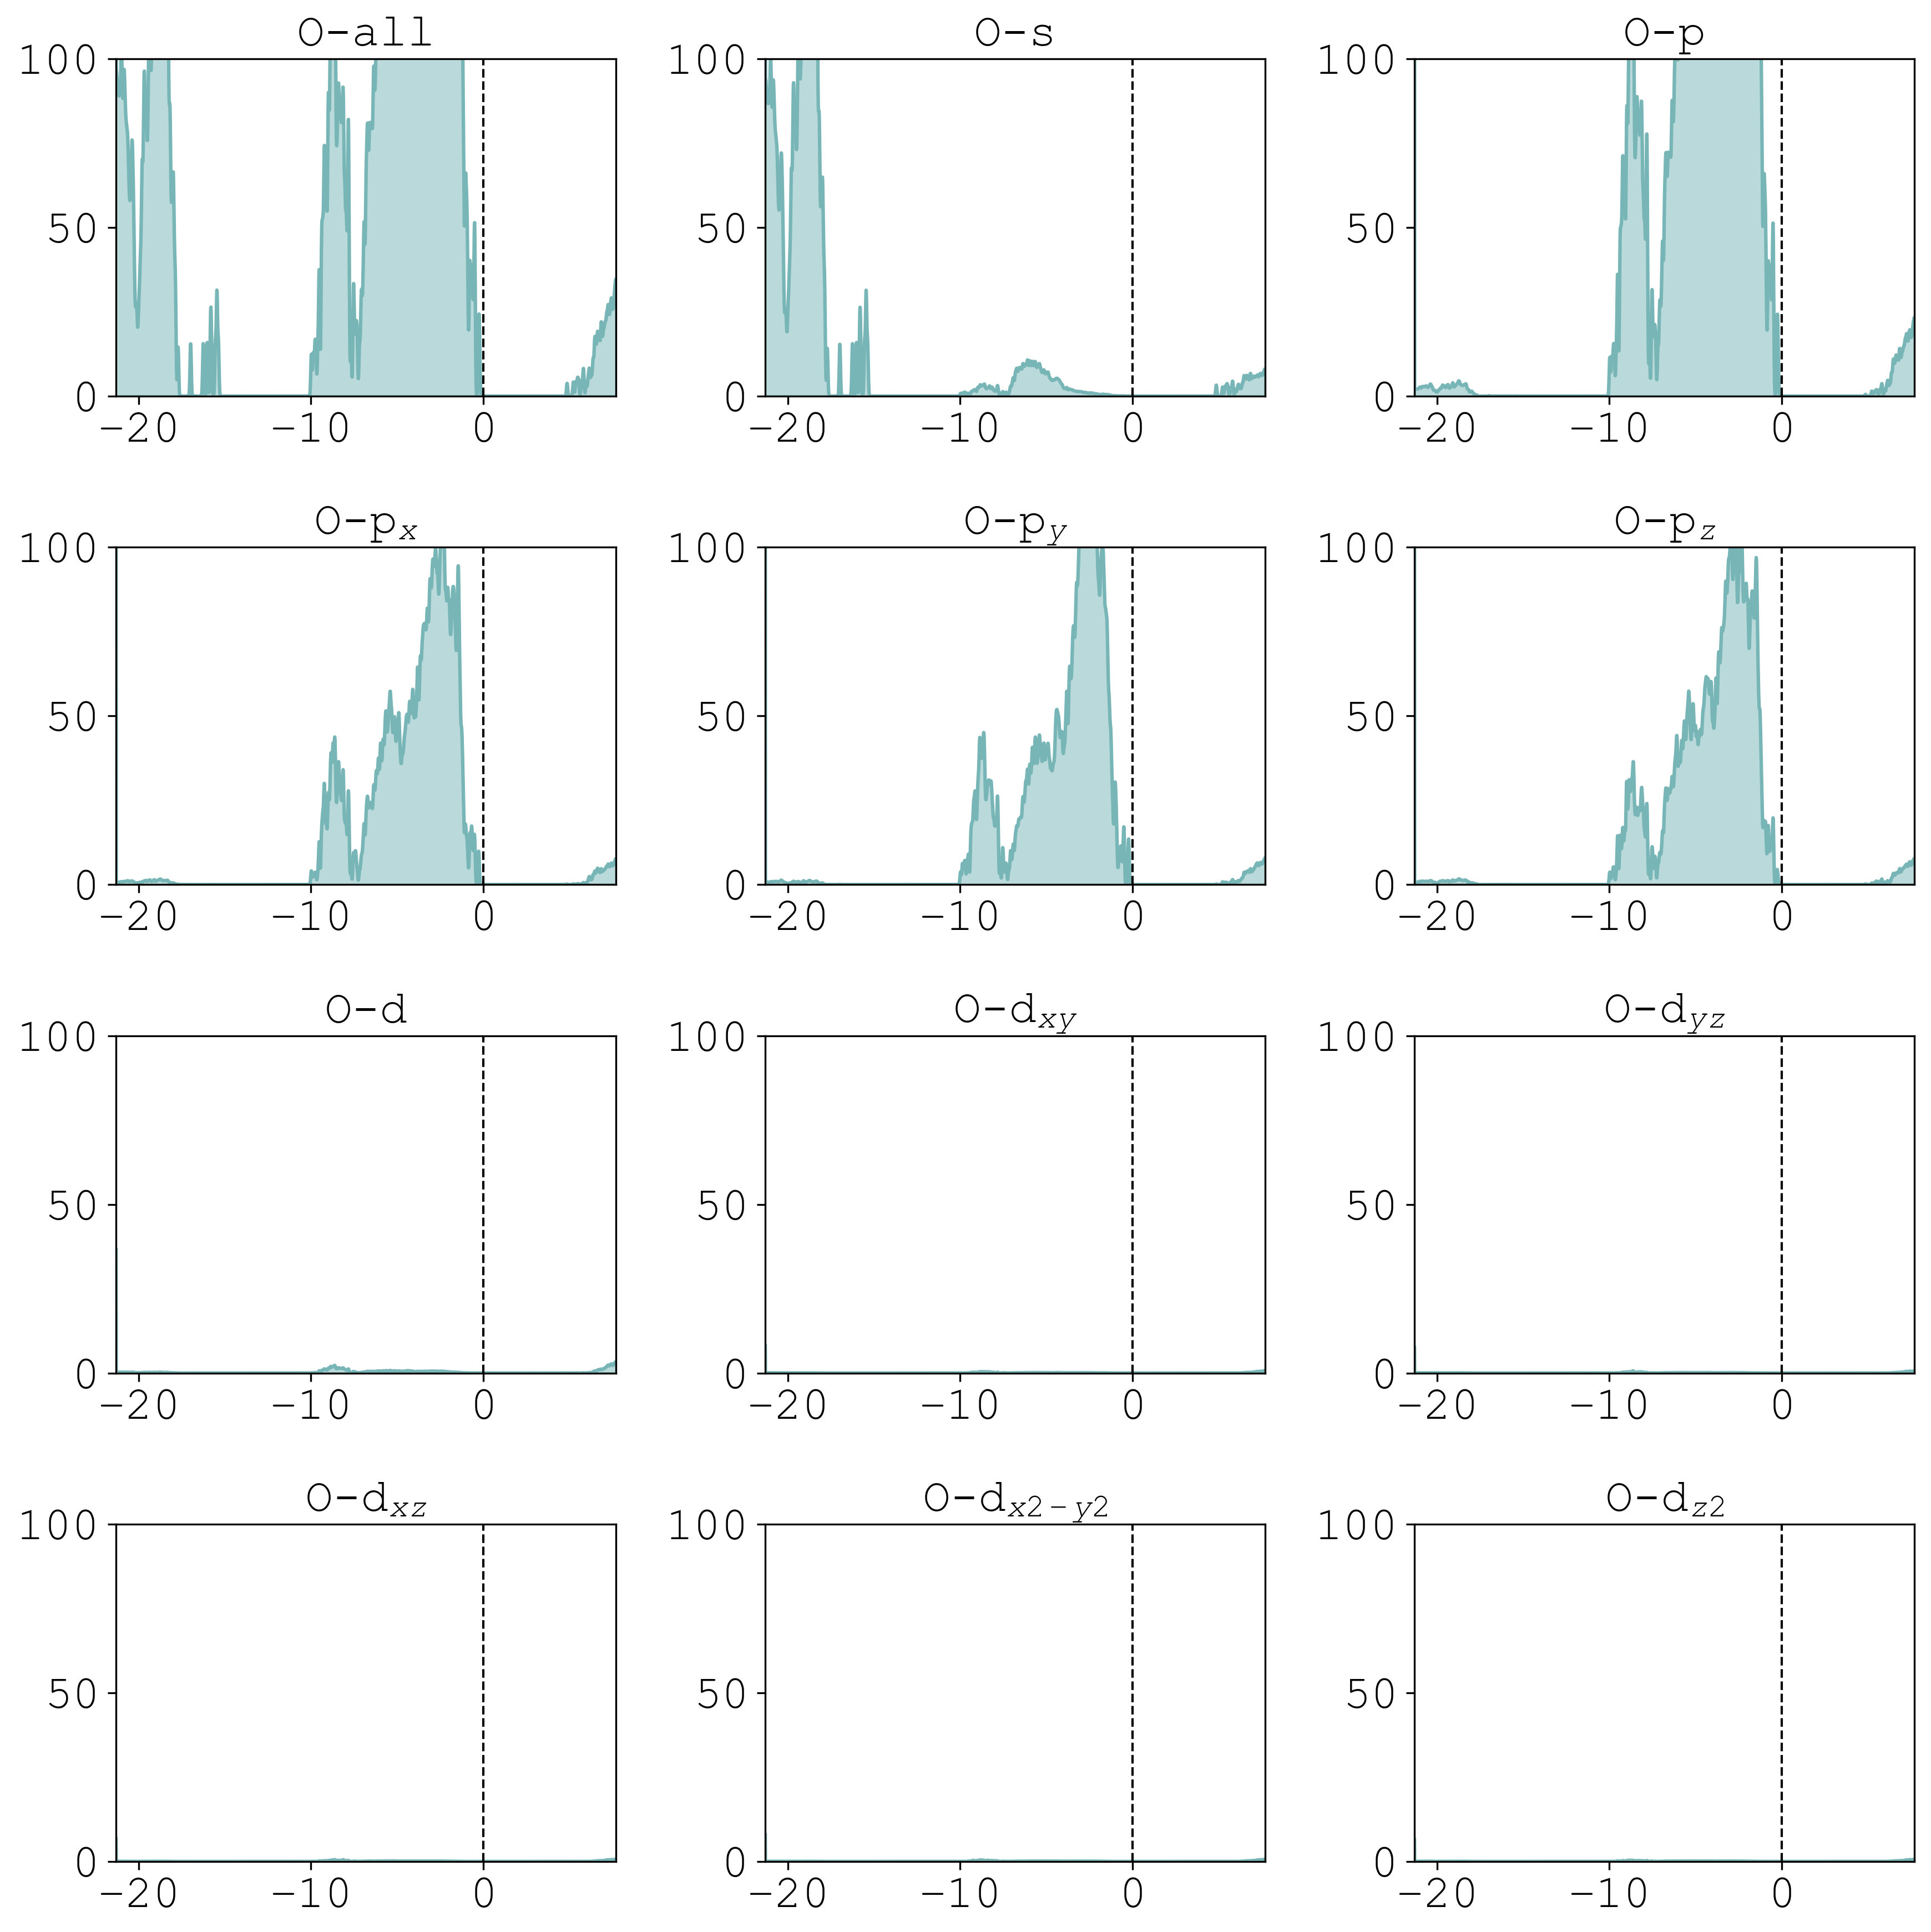
\includegraphics[width=1.0\textwidth]{dos-o-orbitals.png}
    \caption{Orbital-resolved density of states (DOS) for O atoms in C--S--H computed employing the HSEsol hybrid functional. The plots show the total O contribution and its decomposition into \textit{s}, \textit{p} (\textit{p}$_x$, \textit{p}$_y$, \textit{p}$_z$), and \textit{d} (\textit{d}$_{xy}$, \textit{d}$_{yz}$, \textit{d}$_{xz}$, \textit{d}$_{x^2-y^2}$, \textit{d}$_{z^2}$) orbitals. The x-axis reports the energy (in eV) relative to the Fermi level (dashed vertical line at 0 eV), while the y-axis shows the density of states (in states/eV).}
    \label{fig:pdos-o}
\end{figure}
\begin{figure}[h]
    \centering
    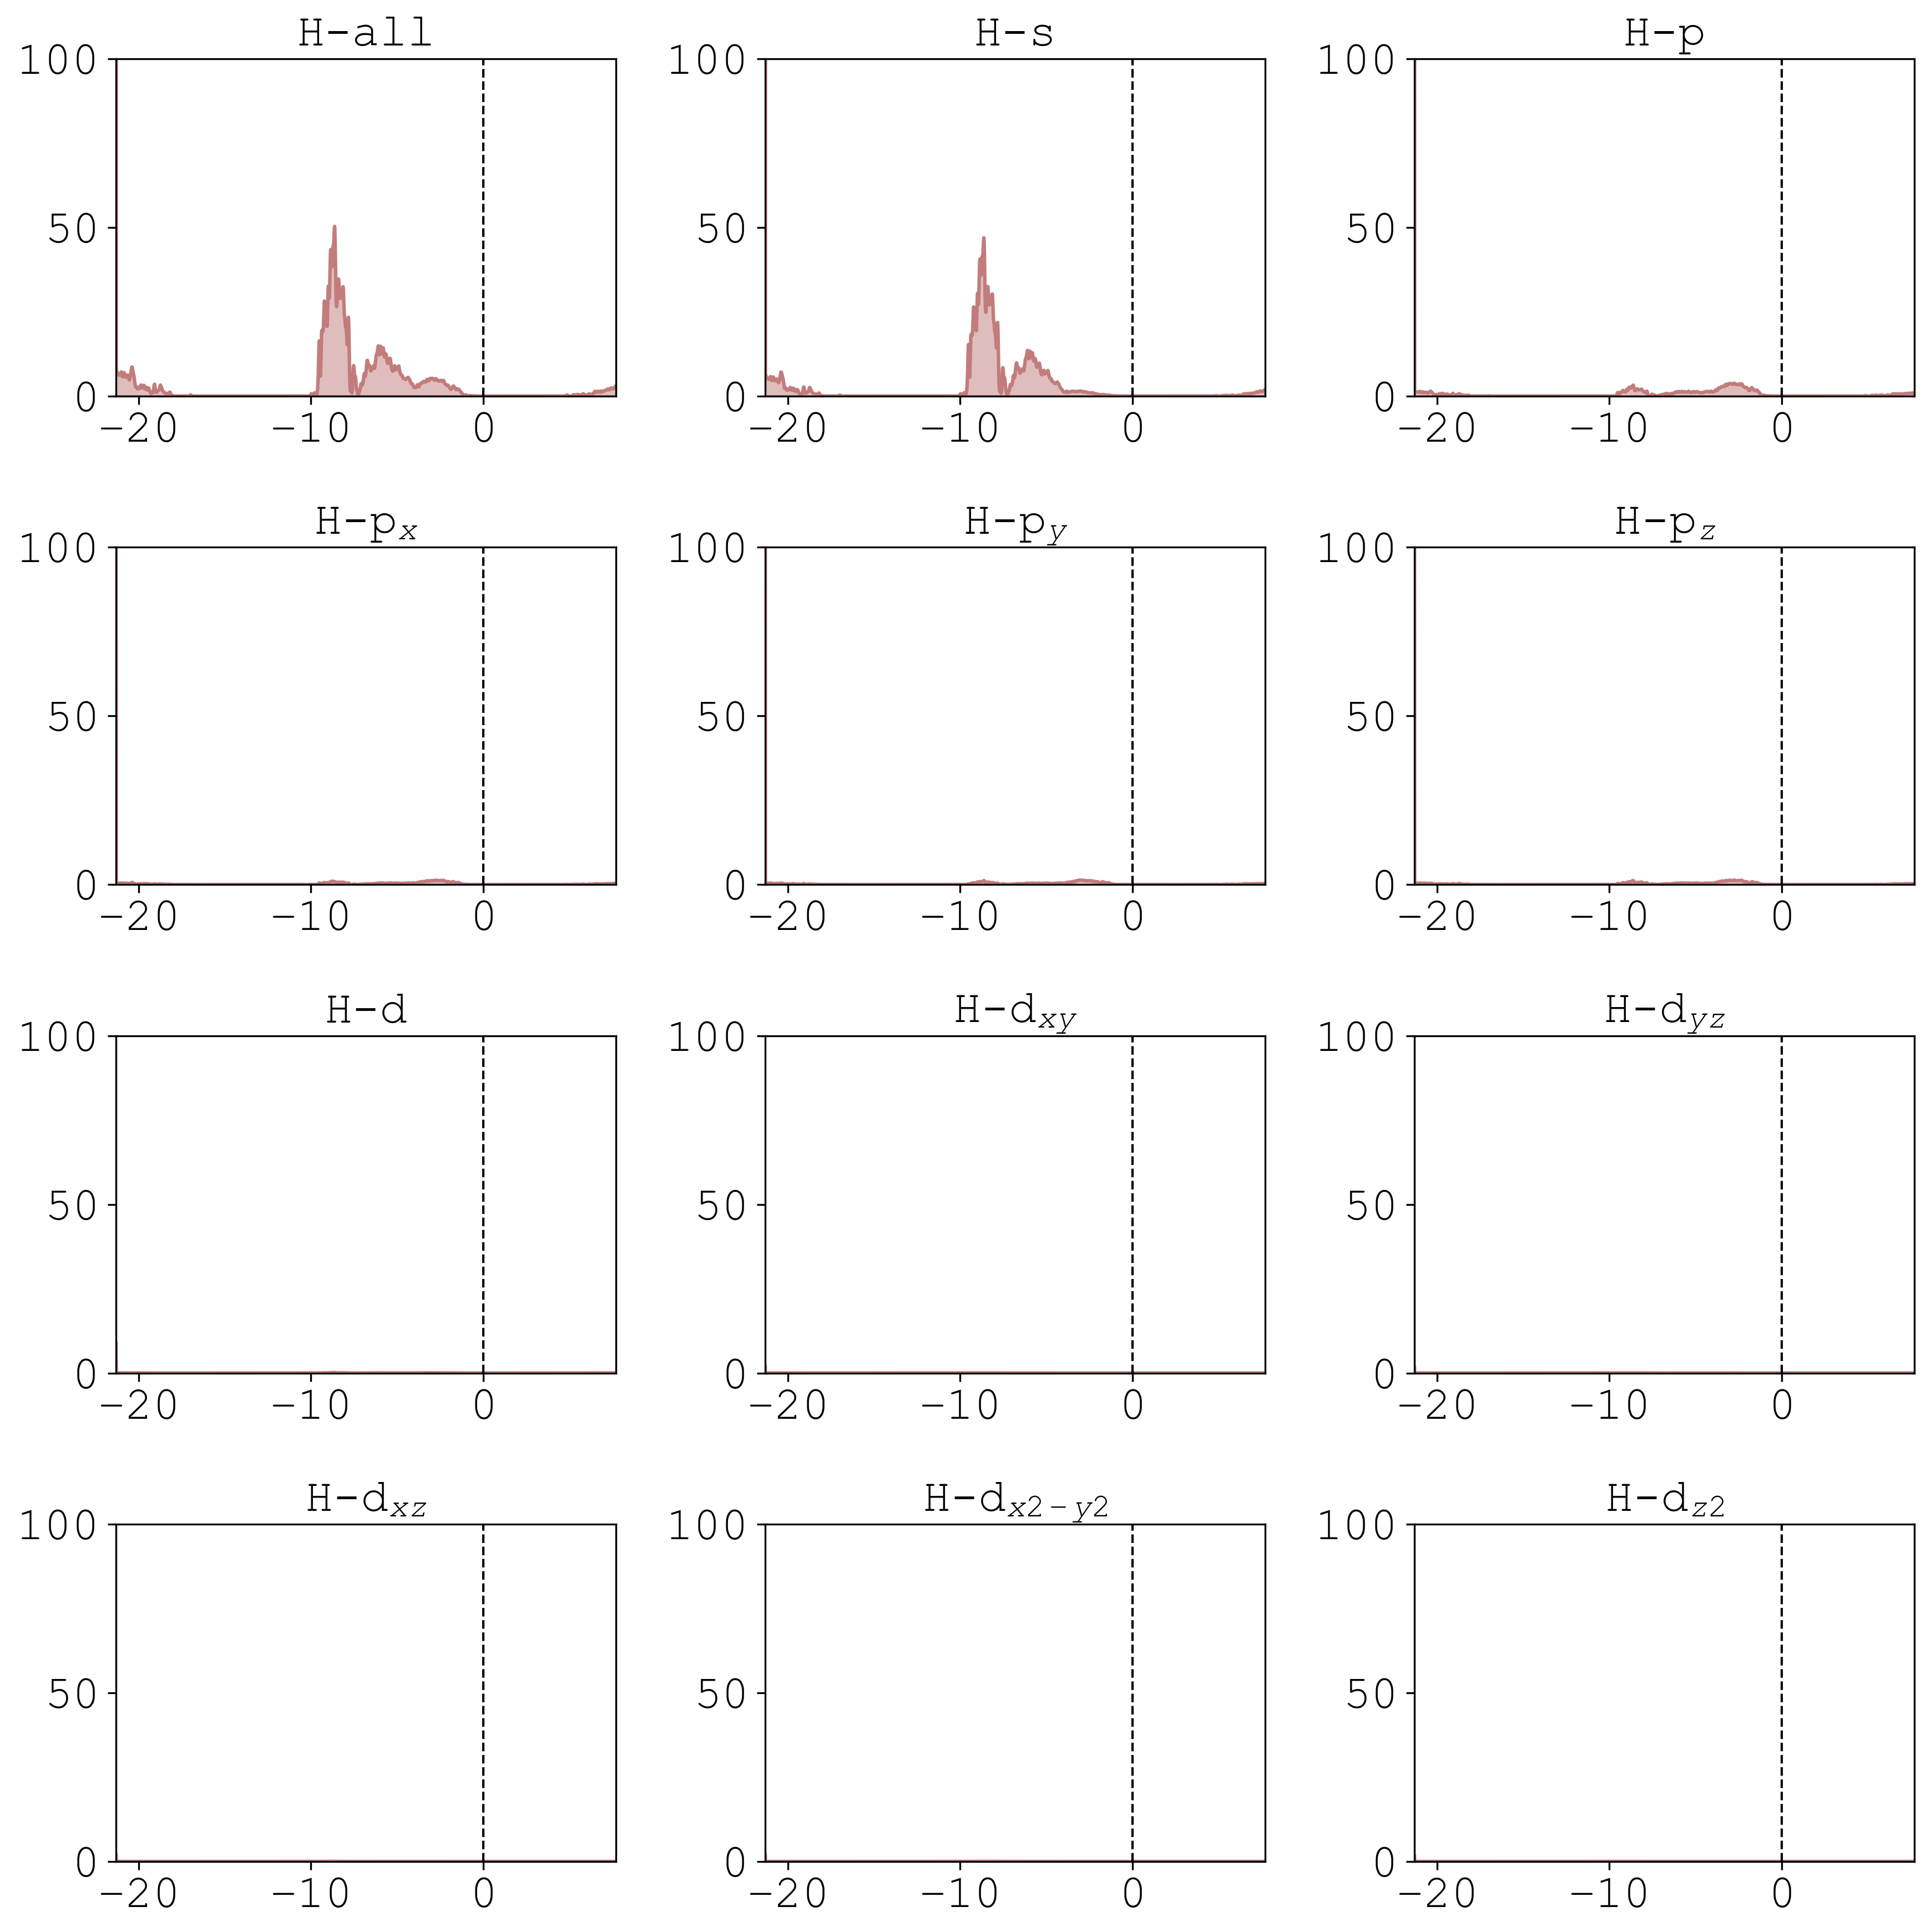
\includegraphics[width=1.0\textwidth]{dos-h-orbitals.png}
    \caption{Orbital-resolved density of states (DOS) for H atoms in C--S--H computed employing the HSEsol hybrid functional. The plots show the total H contribution and its decomposition into \textit{s}, \textit{p} (\textit{p}$_x$, \textit{p}$_y$, \textit{p}$_z$), and \textit{d} (\textit{d}$_{xy}$, \textit{d}$_{yz}$, \textit{d}$_{xz}$, \textit{d}$_{x^2-y^2}$, \textit{d}$_{z^2}$) orbitals. The x-axis reports the energy (in eV) relative to the Fermi level (dashed vertical line at 0 eV), while the y-axis shows the density of states (in states/eV).}
    \label{fig:pdos-h}
\end{figure}

\chapter{Computational Parameters} % Main appendix title
\label{AppendixB} % For referencing this appendix elsewhere, use \ref{AppendixA}

\begin{figure}[H]  
	\centering  
	\begin{threeparttable}  
		\caption{Complete \texttt{INCAR} configuration used for C--S--H structure relaxation. Electronic optimisation is performed with a plane-wave cutoff of 800~eV (\texttt{ENCUT=800}), Gaussian smearing (\texttt{ISMEAR=0}, \texttt{SIGMA=0.05~eV}), and the RMM-DIIS algorithm (\texttt{ALGO=F}) with a charge mixing parameter of 0.1 (\texttt{AMIX=0.1}). Exchange-correlation is treated with the PBEsol functional (\texttt{GGA=PS}) including DFT-D3 zero-damping van der Waals corrections (\texttt{IVDW=11}) and non-spherical contributions (\texttt{LASPH=.TRUE.}). Ionic relaxation uses the conjugate-gradient method (\texttt{IBRION=2}) with full cell relaxation (\texttt{ISIF=3}), a maximum of 700 steps (\texttt{NSW=700}), and a force convergence criterion of 0.02~eV/\AA\ (\texttt{EDIFFG=-0.02}). Additional grid refinement (\texttt{ADDGRID=.TRUE.}) is enabled for improved accuracy.} 
		\label{fig:incar}  
		\resizebox{\textwidth}{!}{  
			\begin{tabular}{>{\columncolor{blue!10}}l>{\columncolor{blue!10}}l>{\columncolor{blue!10}}l>{\columncolor{blue!10}}l>{\columncolor{blue!10}}l>{\columncolor{blue!10}}l>{\columncolor{blue!10}}l>{\columncolor{blue!10}}l>{\columncolor{blue!10}}l>{\columncolor{blue!10}}l>{\columncolor{blue!10}}l>{\columncolor{blue!10}}l>{\columncolor{blue!10}}l>{\columncolor{blue!10}}l>{\columncolor{blue!10}}l>{\columncolor{blue!10}}l>{\columncolor{blue!10}}l>{\columncolor{blue!10}}l>{\columncolor{blue!10}}l}  
				\hline   
				\multicolumn{3}{c}{\cellcolor{blue!10} \textbf{GENERAL}} & & & & & & & & & & & & & & & & \\   
				\textbf{SYSTEM} & \textbf{=  C--S--H} & \textit{\# System name} & & & & & & & & & & & & & & & & \\   
				\textbf{PREC}   & \textbf{= Accurate} & \textit{\# Precision level} & & & & & & & & & & & & & & & & \\   
				\multicolumn{3}{c}{\cellcolor{blue!10} \textbf{ELECTRONIC OPTIMIZATION}} & & & & & & & & & & & & & & & & \\   
				\textbf{ENCUT}  & \textbf{= 800} & \textit{\# Plane-wave cutoff (eV)} & & & & & & & & & & & & & & & & \\   
				\textbf{LREAL}  & \textbf{= Auto} & \textit{\# Real-space projection} & & & & & & & & & & & & & & & & \\   
				\textbf{ISMEAR} & \textbf{= 0} & \textit{\# Smearing method} & & & & & & & & & & & & & & & & \\   
				\textbf{SIGMA}  & \textbf{= 0.05} & \textit{\# Smearing width (eV)} & & & & & & & & & & & & & & & & \\   
				\textbf{ALGO}   & \textbf{= F} & \textit{\# Electronic minimization algorithm} & & & & & & & & & & & & & & & & \\   
				\textbf{AMIX}   & \textbf{= 0.1} & \textit{\# Charge density mixing parameter (damping)} & & & & & & & & & & & & & & & & \\   
				\multicolumn{3}{c}{\cellcolor{blue!10} \textbf{EXCHANGE-CORRELATION / FUNCTIONAL}} & & & & & & & & & & & & & & & & \\   
				\textbf{GGA}    & \textbf{= PS} & \textit{\# PBEsol functional} & & & & & & & & & & & & & & & & \\   
				\textbf{IVDW}   & \textbf{= 11} & \textit{\# DFT-D3(zero) vdW correction} & & & & & & & & & & & & & & & & \\   
				\textbf{LASPH}  & \textbf{= .TRUE.} & \textit{\# Non-spherical contributions} & & & & & & & & & & & & & & & & \\   
				\textbf{LMAXMIX}& \textbf{= 4} & \textit{\# Maximum l for charge mixing} & & & & & & & & & & & & & & & & \\   
				\multicolumn{3}{c}{\cellcolor{blue!10} \textbf{CHARGE \& WAVEFUNCTION}} & & & & & & & & & & & & & & & & \\   
				\textbf{LCHARG} & \textbf{= F} & \textit{\# Do not write CHGCAR} & & & & & & & & & & & & & & & & \\   
				\multicolumn{3}{c}{\cellcolor{blue!10} \textbf{IONIC RELAXATION}} & & & & & & & & & & & & & & & & \\   
				\textbf{NELMIN} & \textbf{= 4} & \textit{\# Minimum SCF steps} & & & & & & & & & & & & & & & & \\   
				\textbf{MAXMIX} & \textbf{= 40} & \textit{\# Maximum mixing steps} & & & & & & & & & & & & & & & & \\   
				\textbf{IBRION} & \textbf{= 2} & \textit{\# Ionic relaxation algorithm} & & & & & & & & & & & & & & & & \\   
				\textbf{ISIF}   & \textbf{= 3} & \textit{\# Relax ions + cell shape + volume} & & & & & & & & & & & & & & & & \\   
				\textbf{NSW}    & \textbf{= 700} & \textit{\# Maximum ionic steps} & & & & & & & & & & & & & & & & \\   
				\textbf{EDIFFG} & \textbf{= -0.02} & \textit{\# Convergence criterion (eV/\AA)} & & & & & & & & & & & & & & & & \\   
				\textbf{ADDGRID}& \textbf{= T} & \textit{\# Additional grid for accuracy} & & & & & & & & & & & & & & & & \\   
				\hline  
			\end{tabular}  
		}  
	\end{threeparttable}  
\end{figure}


\begin{figure}[H]  
    \centering  
    \begin{threeparttable}  
        \caption{INCAR configuration used for density of states (DOS) calculations of C--S--H. Electronic optimisation uses a plane-wave cutoff of 800~eV (\texttt{ENCUT=800}), Gaussian smearing for insulators (\texttt{ISMEAR=0}, \texttt{SIGMA=0.05~eV}), up to 300 SCF steps (\texttt{NELM=300}), and the Normal blocked-Davidson algorithm (\texttt{ALGO=N}). The HSEsol hybrid functional is applied (\texttt{LHFCALC=.TRUE.}) with 25\% exact exchange (\texttt{AEXX=0.25}) and screening parameter (\texttt{HFSCREEN=0.2}). DFT-D3 dispersion corrections are included (\texttt{IVDW=11}) with parameters (\texttt{VDW\_S8=0.7220}) and (\texttt{VDW\_SR=1.5810}). DOS output is defined by (\texttt{NEDOS=3001}) points in the energy range from -19.0 to 10.0~eV (\texttt{EMIN=-19.0}, \texttt{EMAX=10.0}). Ionic relaxation is disabled (\texttt{NSW=0}, \texttt{IBRION=-1}).}
        \label{fig:incar_dos}  
        \resizebox{\textwidth}{!}{  
            \begin{tabular}{
                >{\columncolor{blue!10}}l
                >{\columncolor{blue!10}}l
                >{\columncolor{blue!10}}l
                >{\columncolor{blue!10}}l
                >{\columncolor{blue!10}}l
                >{\columncolor{blue!10}}l
                >{\columncolor{blue!10}}l
                >{\columncolor{blue!10}}l
                >{\columncolor{blue!10}}l
                >{\columncolor{blue!10}}l
                >{\columncolor{blue!10}}l
                >{\columncolor{blue!10}}l
                >{\columncolor{blue!10}}l
                >{\columncolor{blue!10}}l
                >{\columncolor{blue!10}}l
                >{\columncolor{blue!10}}l
                >{\columncolor{blue!10}}l
                >{\columncolor{blue!10}}l
                >{\columncolor{blue!10}}l}  

                \hline  
                \multicolumn{3}{c}{\cellcolor{blue!10}\textbf{GENERAL SETTINGS}} & & & & & & & & & & & & & & & &\\  
                \textbf{SYSTEM} & \textbf{= CSH-DOS} & \textit{\# System name} & & & & & & & & & & & & & & & & \\  

                \multicolumn{3}{c}{\cellcolor{blue!10}\textbf{ELECTRONIC RX}} & & & & & & & & & & & & & & & & \\  
                \textbf{ISMEAR} & \textbf{= 0} & \textit{\# Gaussian smearing (insulators)} & & & & & & & & & & & & & & & & \\  
                \textbf{SIGMA}  & \textbf{= 0.05} & \textit{\# Smearing width (eV)} & & & & & & & & & & & & & & & & \\  
                \textbf{LREAL}  & \textbf{= Auto} & \textit{\# Projection in real space} & & & & & & & & & & & & & & & & \\  
                \textbf{PREC}   & \textbf{= Accurate} & \textit{\# Precision level} & & & & & & & & & & & & & & & & \\  
                \textbf{ENCUT}  & \textbf{= 800} & \textit{\# Plane-wave cutoff energy} & & & & & & & & & & & & & & & & \\  
                \textbf{ALGO}   & \textbf{= N} & \textit{\# Electronic minimization algorithm} & & & & & & & & & & & & & & & & \\  
                \textbf{NELM}   & \textbf{= 300} & \textit{\# Max SCF steps} & & & & & & & & & & & & & & & & \\  
                \textbf{EDIFF}  & \textbf{= 5E-5} & \textit{\# Electronic energy convergence} & & & & & & & & & & & & & & & & \\  
                \textbf{LORBIT} & \textbf{= 11} & \textit{\# Projected DOS output} & & & & & & & & & & & & & & & & \\  

                \multicolumn{3}{c}{\cellcolor{blue!10}\textbf{FUNCTIONAL}} & & & & & & & & & & & & & & & & \\  
                \textbf{GGA}    & \textbf{= PS} & \textit{\# PBEsol base for HSEsol} & & & & & & & & & & & & & & & & \\  
                \textbf{LHFCALC} & \textbf{= .TRUE.} & \textit{\# Enable hybrid Hartree-Fock exchange} & & & & & & & & & & & & & & & & \\  
                \textbf{HFSCREEN} & \textbf{= 0.2} & \textit{\# HSE screening parameter} & & & & & & & & & & & & & & & & \\  
                \textbf{AEXX}    & \textbf{= 0.25} & \textit{\# Fraction of exact exchange} & & & & & & & & & & & & & & & & \\  

                \multicolumn{3}{c}{\cellcolor{blue!10}\textbf{DISPERSION \& PAW SETTINGS}} & & & & & & & & & & & & & & & & \\  
                \textbf{IVDW}    & \textbf{= 11} & \textit{\# D3 dispersion correction} & & & & & & & & & & & & & & & & \\  
                \textbf{LASPH}   & \textbf{= .TRUE.} & \textit{\# Non-spherical PAW contributions} & & & & & & & & & & & & & & & & \\  
                \textbf{LMAXMIX} & \textbf{= 4} & \textit{\# Max l quantum number} & & & & & & & & & & & & & & & & \\  
                \textbf{VDW\_S8} & \textbf{= 0.7220} & & & & & & & & & & & & & & & & & \\  
                \textbf{VDW\_SR} & \textbf{= 1.5810} & & & & & & & & & & & & & & & & & \\  

                \multicolumn{3}{c}{\cellcolor{blue!10}\textbf{CHARGE \& WAVEFUNCTIONS}} & & & & & & & & & & & & & & & & \\  
                \textbf{ICHARG} & \textbf{= 2} & \textit{\# Full SCF calculation} & & & & & & & & & & & & & & & & \\  
                \textbf{LCHARG} & \textbf{= .TRUE.} & \textit{\# Write CHGCAR} & & & & & & & & & & & & & & & & \\  
                \textbf{LWAVE}  & \textbf{= .FALSE.} & \textit{\# Do not write WAVECAR} & & & & & & & & & & & & & & & & \\  

                \multicolumn{3}{c}{\cellcolor{blue!10}\textbf{DOS SETTINGS}} & & & & & & & & & & & & & & & & \\  
                \textbf{NEDOS} & \textbf{= 3001} & \textit{\# Number of DOS points} & & & & & & & & & & & & & & & & \\  
                \textbf{EMIN}  & \textbf{= -19.0} & \textit{\# Minimum energy (eV)} & & & & & & & & & & & & & & & & \\  
                \textbf{EMAX}  & \textbf{= 10.0} & \textit{\# Maximum energy (eV)} & & & & & & & & & & & & & & & & \\  

                \multicolumn{3}{c}{\cellcolor{blue!10}\textbf{IONIC RELAXATION}} & & & & & & & & & & & & & & & & \\  
                \textbf{NSW}   & \textbf{= 0} & \textit{\# No ionic relaxation} & & & & & & & & & & & & & & & & \\  
                \textbf{IBRION} & \textbf{= -1} & \textit{\# No ionic steps} & & & & & & & & & & & & & & & & \\  

                \multicolumn{3}{c}{\cellcolor{blue!10}\textbf{OTHER SETTINGS}} & & & & & & & & & & & & & & & & \\  
                \textbf{BANDGAP} & \textbf{= COMPACT} & & & & & & & & & & & & & & & & & \\  
                \textbf{NCORE} & \textbf{= 24} & \textit{\# Cores per node} & & & & & & & & & & & & & & & & \\  
                \textbf{NSIM}  & \textbf{= 6} & \textit{\# Parallelization parameter} & & & & & & & & & & & & & & & & \\  
                %\textbf{KPAR} & \textbf{= 2} & & & & & & & & & & & & & & & & & \\  

                \hline  
            \end{tabular}  
        }  
    \end{threeparttable}  
\end{figure}

\begin{figure}[H]
    \centering
    \begin{threeparttable}
        \caption{INCAR configuration used for ab initio molecular dynamics (AIMD) simulations of C--S--H, simultaneously for machine learning force field (MLFF) training. Ionic dynamics employ the velocity-Verlet algorithm (\texttt{IBRION=0}) for 50,000 steps (\texttt{NSW=50000}) with a timestep of 2~fs (\texttt{POTIM=2.0}). A Langevin thermostat is applied with damping (\texttt{LANGEVIN\_GAMMA=1}) and (\texttt{LANGEVIN\_GAMMA\_L=10}), targeting an initial temperature of 400~K (\texttt{TEBEG=400}). Electronic optimization uses a plane-wave cutoff of 800~eV (\texttt{ENCUT=800}), Gaussian smearing for insulators (\texttt{ISMEAR=0}, \texttt{SIGMA=0.05~eV}), and the Normal blocked-Davidson algorithm (\texttt{ALGO=N}) with convergence (\texttt{EDIFF=1E-5}). The PBEsol functional is applied with non-spherical contributions (\texttt{LASPH=.TRUE.}) and (\texttt{LMAXMIX=4}). Periodic cell relaxation is allowed (\texttt{ISIF=3}). Machine learning force field training is enabled (\texttt{ML\_LMLFF=.TRUE.}, \texttt{ML\_MODE=TRAIN}).}
        \label{fig:incar_md}
        \resizebox{\textwidth}{!}{
            \begin{tabular}{>{\columncolor{blue!10}}l>{\columncolor{blue!10}}l>{\columncolor{blue!10}}l>{\columncolor{blue!10}}l>{\columncolor{blue!10}}l>{\columncolor{blue!10}}l>{\columncolor{blue!10}}l>{\columncolor{blue!10}}l>{\columncolor{blue!10}}l>{\columncolor{blue!10}}l>{\columncolor{blue!10}}l>{\columncolor{blue!10}}l>{\columncolor{blue!10}}l>{\columncolor{blue!10}}l>{\columncolor{blue!10}}l>{\columncolor{blue!10}}l>{\columncolor{blue!10}}l>{\columncolor{blue!10}}l>{\columncolor{blue!10}}l}
                \hline
                \multicolumn{3}{c}{\cellcolor{blue!10} \textbf{GENERAL}} & & & & & & & & & & & & & & & & \\
                \textbf{SYSTEM} & \textbf{= C--S--H} & & & & & & & & & & & & & & & & & \\
                \multicolumn{3}{c}{\cellcolor{blue!10} \textbf{ELECTRONIC OPTIMIZATION}} & & & & & & & & & & & & & & & & \\
                \textbf{ENCUT}  & \textbf{= 800}  &  & & & & & & & & & & & & & & & & \\
                \textbf{LREAL}  & \textbf{= auto} &  & & & & & & & & & & & & & & & & \\
                \textbf{ISMEAR} & \textbf{= 0}    &  & & & & & & & & & & & & & & & & \\
                \textbf{SIGMA}  & \textbf{= 0.05} & & & & & & & & & & & & & & & & & \\
                \textbf{ALGO}   & \textbf{= N} & & & & & & & & & & & & & & & & & \\
                \textbf{EDIFF}  & \textbf{= 1E-5} & & & & & & & & & & & & & & & & & \\
                \multicolumn{3}{c}{\cellcolor{blue!10} \textbf{EXCHANGE-CORRELATION / FUNCTIONAL}} & & & & & & & & & & & & & & & & \\
                \textbf{GGA}    & \textbf{= PS} & & & & & & & & & & & & & & & & & \\
                \textbf{LASPH}  & \textbf{= .TRUE.} & & & & & & & & & & & & & & & & & \\
                \textbf{LMAXMIX}& \textbf{= 4} & & & & & & & & & & & & & & & & & \\
                \multicolumn{3}{c}{\cellcolor{blue!10} \textbf{CHARGE \& WAVEFUNCTION}} & & & & & & & & & & & & & & & & \\
                \textbf{LWAVE}  & \textbf{= F} & & & & & & & & & & & & & & & & & \\
                \textbf{LCHARG} & \textbf{= F} & & & & & & & & & & & & & & & & & \\
                \multicolumn{3}{c}{\cellcolor{blue!10} \textbf{MOLECULAR DYNAMICS}} & & & & & & & & & & & & & & & & \\
                \textbf{IBRION} & \textbf{= 0} & & & & & & & & & & & & & & & & & \\
                \textbf{NSW}    & \textbf{= 50000} & & & & & & & & & & & & & & & & & \\
                \textbf{POTIM}  & \textbf{= 2.0} & & & & & & & & & & & & & & & & & \\
                \textbf{MDALGO} & \textbf{= 3} & & & & & & & & & & & & & & & & & \\
                \textbf{LANGEVIN\_GAMMA} & \textbf{= 1 1 1 1} & & & & & & & & & & & & & & & & & \\
                \textbf{LANGEVIN\_GAMMA\_L} & \textbf{= 10} & & & & & & & & & & & & & & & & & \\
                \textbf{PMASS}  & \textbf{= 10} & & & & & & & & & & & & & & & & & \\
                \textbf{TEBEG}  & \textbf{= 400} & & & & & & & & & & & & & & & & & \\
                \textbf{POMASS} & \textbf{= 40.078 28.085 16.000 8.00} & & & & & & & & & & & & & & & & & \\
                \textbf{ISIF}   & \textbf{= 3} & & & & & & & & & & & & & & & & & \\
                \multicolumn{3}{c}{\cellcolor{blue!10} \textbf{K-POINTS}} & & & & & & & & & & & & & & & & \\
                \textbf{KSPACING} & \textbf{= 1} & & & & & & & & & & & & & & & & & \\
                \multicolumn{3}{c}{\cellcolor{blue!10} \textbf{MACHINE LEARNING}} & & & & & & & & & & & & & & & & \\
                \textbf{ML\_LMLFF} & \textbf{= .TRUE.} & & & & & & & & & & & & & & & & & \\
                \textbf{ML\_MODE}  & \textbf{= TRAIN} & & & & & & & & & & & & & & & & & \\
                \textbf{ML\_WTSIF} & \textbf{= 2} & & & & & & & & & & & & & & & & & \\
                \hline
            \end{tabular}
        }
    \end{threeparttable}
\end{figure}

\begin{figure}[H]
    \centering
    \begin{threeparttable}
        \caption{INCAR configuration used for molecular dynamics (MD) simulations of C--S--H using a machine learning force field (MLFF). Ionic dynamics are performed with the velocity-Verlet algorithm (\texttt{IBRION=0}) for 50,000 steps (\texttt{NSW=50000}) with a timestep of 2~fs (\texttt{POTIM=2.0}). A Langevin thermostat is applied (\texttt{MDALGO=3}) with damping parameters (\texttt{LANGEVIN\_GAMMA=1 1 1 1} and \texttt{LANGEVIN\_GAMMA\_L=10}), targeting an initial temperature of 400~K (\texttt{TEBEG=400}). Full ionic and cell relaxation is enabled (\texttt{ISIF=3}). Machine learning force field usage is controlled via (\texttt{ML\_LMLFF=.TRUE.}, \texttt{ML\_ISTART=2}). Electronic structure parameters are not included since the MD is performed solely with the MLFF.}
        \label{fig:incar_md_parallel}
        \resizebox{\textwidth}{!}{
            \begin{tabular}{>{\columncolor{blue!10}}l>{\columncolor{blue!10}}l>{\columncolor{blue!10}}l>{\columncolor{blue!10}}l>{\columncolor{blue!10}}l>{\columncolor{blue!10}}l>{\columncolor{blue!10}}l>{\columncolor{blue!10}}l>{\columncolor{blue!10}}l>{\columncolor{blue!10}}l>{\columncolor{blue!10}}l>{\columncolor{blue!10}}l>{\columncolor{blue!10}}l>{\columncolor{blue!10}}l>{\columncolor{blue!10}}l>{\columncolor{blue!10}}l>{\columncolor{blue!10}}l>{\columncolor{blue!10}}l>{\columncolor{blue!10}}l}
                \hline
                \multicolumn{3}{c}{\cellcolor{blue!10} \textbf{GENERAL}} & & & & & & & & & & & & & & & & \\
                \textbf{SYSTEM} & \textbf{= C--S--H} & & & & & & & & & & & & & & & & & \\
                \multicolumn{3}{c}{\cellcolor{blue!10} \textbf{MOLECULAR DYNAMICS}} & & & & & & & & & & & & & & & & \\
                \textbf{IBRION} & \textbf{= 0} & & & & & & & & & & & & & & & & & \\
                \textbf{NSW}    & \textbf{= 50000} & & & & & & & & & & & & & & & & & \\
                \textbf{POTIM}  & \textbf{= 2.0} & & & & & & & & & & & & & & & & & \\
                \textbf{MDALGO} & \textbf{= 3} & & & & & & & & & & & & & & & & & \\
                \textbf{LANGEVIN\_GAMMA} & \textbf{= 1 1 1 1} & & & & & & & & & & & & & & & & & \\
                \textbf{LANGEVIN\_GAMMA\_L} & \textbf{= 10} & & & & & & & & & & & & & & & & & \\
                \textbf{PMASS}  & \textbf{= 10} & & & & & & & & & & & & & & & & & \\
                \textbf{TEBEG}  & \textbf{= 400} & & & & & & & & & & & & & & & & & \\
                \textbf{POMASS} & \textbf{= 40.078 28.085 16.000 8.00} & & & & & & & & & & & & & & & & & \\
                \textbf{ISIF}   & \textbf{= 3} & & & & & & & & & & & & & & & & & \\
                \multicolumn{3}{c}{\cellcolor{blue!10} \textbf{K-POINTS}} & & & & & & & & & & & & & & & & \\
                \textbf{KSPACING} & \textbf{= 1} & & & & & & & & & & & & & & & & & \\
                \multicolumn{3}{c}{\cellcolor{blue!10} \textbf{MACHINE LEARNING}} & & & & & & & & & & & & & & & & \\
                \textbf{ML\_LMLFF} & \textbf{= .TRUE.} & & & & & & & & & & & & & & & & & \\
                \textbf{ML\_ISTART} & \textbf{= 2} & & & & & & & & & & & & & & & & & \\
                \multicolumn{3}{c}{\cellcolor{blue!10} \textbf{PARALLELIZATION}} & & & & & & & & & & & & & & & & \\
                \textbf{NCORE}  & \textbf{= 48} & & & & & & & & & & & & & & & & & \\
                \textbf{NSIM}   & \textbf{= 4} & & & & & & & & & & & & & & & & & \\
                \textbf{ISYM}   & \textbf{= 0} & & & & & & & & & & & & & & & & & \\
                \textbf{LSCALU} & \textbf{= .TRUE.} & & & & & & & & & & & & & & & & & \\
                \textbf{LSCALAPACK} & \textbf{= .TRUE.} & & & & & & & & & & & & & & & & & \\
                \hline
            \end{tabular}
        }
    \end{threeparttable}
\end{figure}

% \begin{figure}[h]
%     \centering
%     \begin{threeparttable}
%         \caption{Example of an \texttt{INCAR} file used for molecular dynamics (MD) simulation of cement. This file specifies the MD algorithm, Langevin thermostat parameters, ionic step settings, and machine learning force field parameters. Additional tags may be included or removed based on specific simulation requirements.}
%         \label{fig:incar_md_cement}
%         \resizebox{\textwidth}{!}{
%             \begin{tabular}{>{\columncolor{blue!10}}l>{\columncolor{blue!10}}l>{\columncolor{blue!10}}l>{\columncolor{blue!10}}l>{\columncolor{blue!10}}l>{\columncolor{blue!10}}l>{\columncolor{blue!10}}l>{\columncolor{blue!10}}l>{\columncolor{blue!10}}l>{\columncolor{blue!10}}l>{\columncolor{blue!10}}l>{\columncolor{blue!10}}l>{\columncolor{blue!10}}l>{\columncolor{blue!10}}l>{\columncolor{blue!10}}l>{\columncolor{blue!10}}l>{\columncolor{blue!10}}l>{\columncolor{blue!10}}l>{\columncolor{blue!10}}l}
%                 \hline
%                 \multicolumn{3}{c}{\cellcolor{blue!10} \textbf{GENERAL}} & & & & & & & & & & & & & & & & \\
%                 \textbf{SYSTEM} & \textbf{= cement} & & & & & & & & & & & & & & & & & \\
%                 \multicolumn{3}{c}{\cellcolor{blue!10} \textbf{MOLECULAR DYNAMICS}} & & & & & & & & & & & & & & & & \\
%                 \textbf{IBRION} & \textbf{= 0} & & & & & & & & & & & & & & & & & \\
%                 \textbf{NSW}    & \textbf{= 50000} & & & & & & & & & & & & & & & & & \\
%                 \textbf{POTIM}  & \textbf{= 2.0} & & & & & & & & & & & & & & & & & \\
%                 \textbf{MDALGO} & \textbf{= 3} & & & & & & & & & & & & & & & & & \\
%                 \textbf{LANGEVIN\_GAMMA} & \textbf{= 1 1 1 1} & & & & & & & & & & & & & & & & & \\
%                 \textbf{LANGEVIN\_GAMMA\_L} & \textbf{= 10} & & & & & & & & & & & & & & & & & \\
%                 \textbf{PMASS}  & \textbf{= 10} & & & & & & & & & & & & & & & & & \\
%                 \textbf{TEBEG}  & \textbf{= 400} & & & & & & & & & & & & & & & & & \\
%                 \textbf{POMASS} & \textbf{= 40.078 28.085 16.000 8.00} & & & & & & & & & & & & & & & & & \\
%                 \textbf{ISIF}   & \textbf{= 3} & & & & & & & & & & & & & & & & & \\
%                 \multicolumn{3}{c}{\cellcolor{blue!10} \textbf{K-POINTS}} & & & & & & & & & & & & & & & & \\
%                 \textbf{KSPACING} & \textbf{= 1} & & & & & & & & & & & & & & & & & \\
%                 \multicolumn{3}{c}{\cellcolor{blue!10} \textbf{MACHINE LEARNING}} & & & & & & & & & & & & & & & & \\
%                 \textbf{ML\_LMLFF} & \textbf{= .TRUE.} & & & & & & & & & & & & & & & & & \\
%                 \textbf{ML\_ISTART} & \textbf{= 2} & & & & & & & & & & & & & & & & & \\
%                 \hline
%             \end{tabular}
%         }
%     \end{threeparttable}
% \end{figure}

\begin{figure}[H]
    \centering
    \begin{threeparttable}
        \caption{INCAR configuration used for simulated annealing molecular dynamics (MD) of C--S--H using a machine learning force field (MLFF). Ionic dynamics are performed with the velocity-Verlet algorithm (\texttt{IBRION=0}) for 20,000 steps (\texttt{NSW=20000}) with a timestep of 2~fs (\texttt{POTIM=2.0}). A Langevin thermostat (\texttt{MDALGO=3}) is applied with damping parameters (\texttt{LANGEVIN\_GAMMA=1 1 1 1}, \texttt{LANGEVIN\_GAMMA\_L=10}), starting at \texttt{TEBEG=400~K} and cooling to \texttt{TEEND=0~K}. Full ionic and cell relaxation is enabled (\texttt{ISIF=3}). Machine learning force field usage is controlled via (\texttt{ML\_LMLFF=.TRUE.}, \texttt{ML\_ISTART=2}). Initial conditions correspond to a fresh start of the system (\texttt{ISTART=1}).}
        \label{fig:incar_md_cement_parallel}
        \resizebox{\textwidth}{!}{
            \begin{tabular}{>{\columncolor{blue!10}}l>{\columncolor{blue!10}}l>{\columncolor{blue!10}}l>{\columncolor{blue!10}}l>{\columncolor{blue!10}}l>{\columncolor{blue!10}}l>{\columncolor{blue!10}}l>{\columncolor{blue!10}}l>{\columncolor{blue!10}}l>{\columncolor{blue!10}}l>{\columncolor{blue!10}}l>{\columncolor{blue!10}}l>{\columncolor{blue!10}}l>{\columncolor{blue!10}}l>{\columncolor{blue!10}}l>{\columncolor{blue!10}}l>{\columncolor{blue!10}}l>{\columncolor{blue!10}}l>{\columncolor{blue!10}}l}
                \hline
                \multicolumn{3}{c}{\cellcolor{blue!10} \textbf{GENERAL}} & & & & & & & & & & & & & & & & \\
                \textbf{SYSTEM} & \textbf{= cement} & & & & & & & & & & & & & & & & & \\
                \multicolumn{3}{c}{\cellcolor{blue!10} \textbf{MOLECULAR DYNAMICS}} & & & & & & & & & & & & & & & & \\
                \textbf{IBRION} & \textbf{= 0} & & & & & & & & & & & & & & & & & \\
                \textbf{NSW}    & \textbf{= 20000} & & & & & & & & & & & & & & & & & \\
                \textbf{POTIM}  & \textbf{= 2.0} & & & & & & & & & & & & & & & & & \\
                \textbf{MDALGO} & \textbf{= 3} & & & & & & & & & & & & & & & & & \\
                \textbf{LANGEVIN\_GAMMA} & \textbf{= 1 1 1 1} & & & & & & & & & & & & & & & & & \\
                \textbf{LANGEVIN\_GAMMA\_L} & \textbf{= 10} & & & & & & & & & & & & & & & & & \\
                \textbf{PMASS}  & \textbf{= 10} & & & & & & & & & & & & & & & & & \\
                \textbf{TEBEG}  & \textbf{= 400} & & & & & & & & & & & & & & & & & \\
                \textbf{TEEND}  & \textbf{= 0} & & & & & & & & & & & & & & & & & \\
                \textbf{POMASS} & \textbf{= 40.078 28.085 16.000 8.00} & & & & & & & & & & & & & & & & & \\
                \textbf{ISIF}   & \textbf{= 3} & & & & & & & & & & & & & & & & & \\
                \multicolumn{3}{c}{\cellcolor{blue!10} \textbf{INITIAL CONDITIONS}} & & & & & & & & & & & & & & & & \\
                \textbf{ISTART} & \textbf{= 1} & & & & & & & & & & & & & & & & & \\
                \textbf{ICHARG} & \textbf{= 1} & & & & & & & & & & & & & & & & & \\
                \multicolumn{3}{c}{\cellcolor{blue!10} \textbf{K-POINTS}} & & & & & & & & & & & & & & & & \\
                \textbf{KSPACING} & \textbf{= 1} & & & & & & & & & & & & & & & & & \\
                \multicolumn{3}{c}{\cellcolor{blue!10} \textbf{MACHINE LEARNING}} & & & & & & & & & & & & & & & & \\
                \textbf{ML\_LMLFF} & \textbf{= .TRUE.} & & & & & & & & & & & & & & & & & \\
                \textbf{ML\_ISTART} & \textbf{= 2} & & & & & & & & & & & & & & & & & \\
                \multicolumn{3}{c}{\cellcolor{blue!10} \textbf{PARALLELIZATION}} & & & & & & & & & & & & & & & & \\
                \textbf{NCORE}  & \textbf{= 48} & & & & & & & & & & & & & & & & & \\
                \textbf{NSIM}   & \textbf{= 4} & & & & & & & & & & & & & & & & & \\
                \textbf{ISYM}   & \textbf{= 0} & & & & & & & & & & & & & & & & & \\
                \textbf{LSCALU} & \textbf{= .TRUE.} & & & & & & & & & & & & & & & & & \\
                \textbf{LSCALAPACK} & \textbf{= .TRUE.} & & & & & & & & & & & & & & & & & \\
                \hline
            \end{tabular}
        }
    \end{threeparttable}
\end{figure}

\begin{figure}[H]
    \centering
    \begin{threeparttable}
        \caption{INCAR configuration used for machine learning refitting of the \texttt{RCUT1} descriptor for C--S--H. K-point spacing is defined by \texttt{KSPACING=1}. Machine learning force field usage is enabled (\texttt{ML\_LMLFF=.TRUE.}) with the refitting mode (\texttt{ML\_MODE=refit}). The \texttt{ML\_RCUT1} parameter defines the cutoff radius for the \texttt{RCUT1} descriptor and is evaluated over a range of values during the refitting process.}
        \label{fig:incar_mip_rcut1}
        \resizebox{\textwidth}{!}{
            \begin{tabular}{>{\columncolor{blue!10}}l>{\columncolor{blue!10}}l>{\columncolor{blue!10}}l>{\columncolor{blue!10}}l>{\columncolor{blue!10}}l>{\columncolor{blue!10}}l>{\columncolor{blue!10}}l>{\columncolor{blue!10}}l>{\columncolor{blue!10}}l>{\columncolor{blue!10}}l>{\columncolor{blue!10}}l>{\columncolor{blue!10}}l>{\columncolor{blue!10}}l>{\columncolor{blue!10}}l>{\columncolor{blue!10}}l>{\columncolor{blue!10}}l>{\columncolor{blue!10}}l>{\columncolor{blue!10}}l>{\columncolor{blue!10}}l}
                \hline
                \multicolumn{3}{c}{\cellcolor{blue!10} \textbf{GENERAL}} & & & & & & & & & & & & & & & & \\
                \textbf{SYSTEM} & \textbf{= C--S--H} & \textit{\# System name} & & & & & & & & & & & & & & & & \\
                \multicolumn{3}{c}{\cellcolor{blue!10} \textbf{K-POINTS}} & & & & & & & & & & & & & & & & \\
                \textbf{KSPACING} & \textbf{= 1} & \textit{\# K-point spacing} & & & & & & & & & & & & & & & & \\
                \multicolumn{3}{c}{\cellcolor{blue!10} \textbf{MACHINE LEARNING}} & & & & & & & & & & & & & & & & \\
                \textbf{ML\_LMLFF} & \textbf{= .TRUE.} & \textit{\# Enable machine learning force field} & & & & & & & & & & & & & & & & \\
                \textbf{ML\_MODE} & \textbf{= refit} & \textit{\# Machine learning mode} & & & & & & & & & & & & & & & & \\
                \textbf{ML\_RCUT1} & \textbf{= 60.0} & \textit{\# Cutoff radius for rcut1} & & & & & & & & & & & & & & & & \\
                \hline
            \end{tabular}
        }
    \end{threeparttable}
\end{figure}

\begin{figure}[H]
    \centering
    \begin{threeparttable}
        \caption{INCAR configuration used for machine learning refitting of the \texttt{RCUT2} descriptor for C--S--H. K-point spacing is defined by \texttt{KSPACING=1}. Machine learning force field usage is enabled (\texttt{ML\_LMLFF=.TRUE.}) with the refitting mode (\texttt{ML\_MODE=refit}). The \texttt{ML\_RCUT2} parameter defines the cutoff radius for the \texttt{RCUT2} descriptor and is evaluated over a range of values during the refitting process.}
        \label{fig:incar_mip_rcut2}
        \resizebox{\textwidth}{!}{
            \begin{tabular}{>{\columncolor{blue!10}}l>{\columncolor{blue!10}}l>{\columncolor{blue!10}}l>{\columncolor{blue!10}}l>{\columncolor{blue!10}}l>{\columncolor{blue!10}}l>{\columncolor{blue!10}}l>{\columncolor{blue!10}}l>{\columncolor{blue!10}}l>{\columncolor{blue!10}}l>{\columncolor{blue!10}}l>{\columncolor{blue!10}}l>{\columncolor{blue!10}}l>{\columncolor{blue!10}}l>{\columncolor{blue!10}}l>{\columncolor{blue!10}}l>{\columncolor{blue!10}}l>{\columncolor{blue!10}}l>{\columncolor{blue!10}}l}
                \hline
                \multicolumn{3}{c}{\cellcolor{blue!10} \textbf{GENERAL}} & & & & & & & & & & & & & & & & \\
                \textbf{SYSTEM} & \textbf{= C--S--H} & \textit{\# System name} & & & & & & & & & & & & & & & & \\
                \multicolumn{3}{c}{\cellcolor{blue!10} \textbf{K-POINTS}} & & & & & & & & & & & & & & & & \\
                \textbf{KSPACING} & \textbf{= 1} & \textit{\# K-point spacing} & & & & & & & & & & & & & & & & \\
                \multicolumn{3}{c}{\cellcolor{blue!10} \textbf{MACHINE LEARNING}} & & & & & & & & & & & & & & & & \\
                \textbf{ML\_LMLFF} & \textbf{= .TRUE.} & \textit{\# Enable machine learning force field} & & & & & & & & & & & & & & & & \\
                \textbf{ML\_MODE} & \textbf{= refit} & \textit{\# Machine learning mode} & & & & & & & & & & & & & & & & \\
                \textbf{ML\_RCUT2} & \textbf{= 10.0} & \textit{\# Cutoff radius for rcut2} & & & & & & & & & & & & & & & & \\
                \hline
            \end{tabular}
        }
    \end{threeparttable}
\end{figure}